\fig{fv:o6:simultaneity}{同时线随参考系倾斜，测量运动长度必须重选事件}{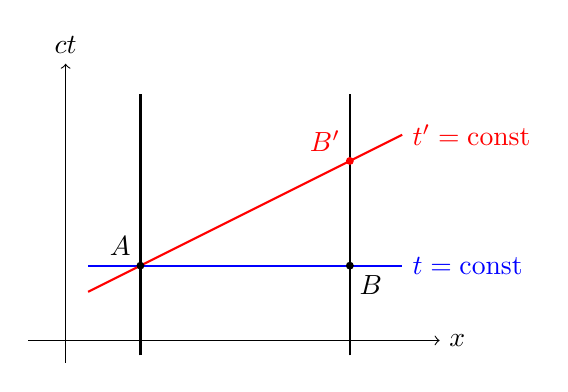
\begin{tikzpicture}[scale=.95]
\draw[->](-.5,0)--(5,0)node[right]{$x$};\draw[->](0,-.3)--(0,3.7)node[above]{$ct$};
\draw[thick](1,-.2)--(1,3.3);\draw[thick](3.8,-.2)--(3.8,3.3);
\draw[blue,thick](.3,1)--(4.5,1)node[right]{$t=\mathrm{const}$};
\draw[red,thick](.3,.65)--(4.5,2.75)node[right]{$t'=\mathrm{const}$};
\fill(1,1)circle(1.5pt)node[above left]{$A$};\fill(3.8,1)circle(1.5pt)node[below right]{$B$};
\fill[red](3.8,2.4)circle(1.5pt)node[above left]{$B'$};
\end{tikzpicture}}
图\ref{fv:o6:simultaneity}把杆画成在 $S$中静止的两条端点世界线。蓝线选出的 $A,B$满足 $\Delta t=0$；变换后却有 $\Delta t'=-\gamma V\Delta x/c^2\ne0$，不能用这对事件直接测量 $S'$中的杆长。$S'$的同时线满足 $ct=(V/c)x+\text{常量}$，应另选同一红线上两端的事件。长度收缩中的“同时测两端”，因而是选事件的条件，不是对同一对任意事件只作空间坐标变换。


图\ref{fv:o6:simultaneity}中杆在 $S$ 静止，故 $x_B-x_A=x_{B'}-x_A=L_0$。红线选取 $A,B'$，满足 $\Delta t'=0$，所以 $\Delta t=VL_0/c^2$。将它代入空间变换：
\[
 L'=\Delta x'=\gamma(L_0-V\Delta t)
 =\gamma L_0(1-\beta^2)=\frac{L_0}{\gamma}.
\]
这与前面“杆在 $S'$ 静止、在 $S$ 运动”的情形互为参照。每一方都在自己的同时线上选端点，所比较的是不同事件对，因而两方都测得对方的运动杆收缩并不矛盾。
